\documentclass[11pt]{beamer}
\usetheme{Warsaw}
\usepackage[utf8]{inputenc}
\usepackage[french]{babel}
\usepackage[T1]{fontenc}
\usepackage{amsmath}
\usepackage{amsfonts}
\usepackage{amssymb}
\usepackage{graphicx}
\usepackage{tikz}
\setbeamertemplate{navigation symbols}{}

\newcommand{\abs}[1]{\left\vert{} #1 \right\vert{}}
\newcommand{\steer}{\textbf{Dirige}}
\newcommand{\steerflat}{\steer^\Delta}
\newcommand{\confspace}{\mathcal{C}}
\newcommand{\qcusp}{q_{\text{cassure}}}

%%%%%%%%%%%%%%%%%%%%%%%%%%%%%%%%%%%%%%%%%%%%%%%%%%%%%%%%%
\author{Théophile \textsc{Bastian}, Kévin \textsc{Le Run}, Rémi \textsc{Oudin}}
\title{HPP \& \og{}Hilare pulling a trailer~\fg}
\date{24 janvier 2017}
%\subject{}
%\logo{}
%\institute{}
\begin{document}

\begin{frame}
	\titlepage{}
\end{frame}

\begin{frame}
    \tableofcontents
\end{frame}

%\begin{frame}
%\tableofcontents
%\end{frame}

% TODO intro : ce qu'on devait faire, pourquoi on l'a pas fait.

\section*{Introduction}

\begin{frame}
    \frametitle{\secname}
    \begin{itemize}
        \item Projet initial~: Implémenter la méthode décrite dans l'article
            ``Motion Planning and Control for Hilare Pulling a Trailer''
            de Laumond et Lamiraux
        \item Utiliser la bibliothèque HPP pour ceci.
        \item Ce qu'on va présenter~:
            \begin{itemize}
                \item Nos échecs pour installer HPP
                \item L'architecture de HPP
                \item L'article sur lequel nous devions travailler
            \end{itemize}
    \end{itemize}
\end{frame}

\section{Problèmes d'installation de HPP}

\subsection{Installation de ROS}

\begin{frame}
    \frametitle{\subsecname}
    \begin{itemize}
        \item Une partie de ROS indigo en dépendance obligatoire.
        \item Indigo est actuellement la version \emph{Old Old Stable} de ROS\@.
        \item Ne fonctionne que sous Ubuntu 12.04 et 14.04
        \item Toute autre distribution est soit expérimentale soit trop moderne
        \item Pas de support pour les versions récentes de Debian
        \item L'installation sous Arch et Xubuntu n'est pas non plus
            fonctionnelle
    \end{itemize}
\end{frame}

\subsubsection{Solutions~?}

\begin{frame}
    \frametitle{\subsecname}
    \begin{enumerate}
        \item Essayé nos machines
        \item Essayé sur un serveur Debian Jessie. ROS ok mais pas HPP\@.
        \item Essayé sur un serveur Ubuntu 12.04. ROS et HPP ok. Enfin c'est ce
            qu'on pensait.
    \end{enumerate}
\end{frame}

\subsection{Installation de HPP}

\begin{frame}[fragile]
    \frametitle{\subsecname}
    \begin{block}{C'est une installation depuis les sources.}
    \begin{itemize}
        \item \url{https://humanoid-path-planner.github.io/hpp-doc/download.html?branch=master}
        \item En théorie, il suffit de télécharger deux fichiers, sourcer un
            des deux, créer les bons dossiers et utiliiser \verb|make|.
    \end{itemize}
    \end{block}
    \begin{alertblock}{Mais.}
        \begin{itemize}
            \item La compilation dure 5 heures. Soit, mais on aimerait avoir un
                ETA.
            \item Cmake, un outil classique de compilation est mis comme
                submodule de tous les dépôts du projet HPP quand bien même le
                guide d'installation demande de l'installer.
            \item L'installation packet par packet n'est pas documentée.
        \end{itemize}
    \end{alertblock}
\end{frame}

\begin{frame}
    \frametitle{Après l'installation}
    En fait, l'installation n'est pas tout à fait suffisante\dots\\
    En effet, même après une installation ``réussie'', ça ne fonctionne pas.
    Plusieurs soucis~:
    \begin{itemize}
        \item Il reste quelques fichiers à sourcer à la main~: Presque normal.
        \item Le Python généré n'est pas tout le temps valide.
        \item Il y a de soucis d'utilisation du serveur X.
        \item Par exemple, l'affichage graphique du  tutoriel fourni ne
            fonctionne pas.
        \item Problème de dbus ?
    \end{itemize}
\end{frame}
\section{Architecture de HPP}

\begin{frame}
    \begin{figure}
        \begin{center}
            \begin{tikzpicture}
                \node at (0,1)
                {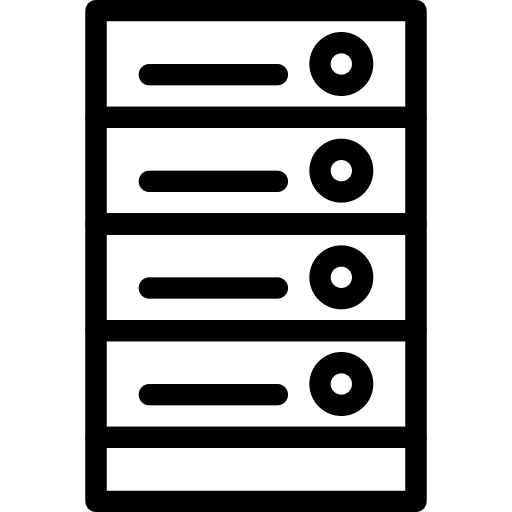
\includegraphics[width=0.1\textwidth]{server_icon.png}};
                \node[rectangle, draw] (c) at (0,0) {CORBA};
                \onslide<2->{%
                    \node[rectangle, draw] (r) at (4,2) {Robots};
                    \node[rectangle, draw] (o) at (4,0) {Obstacles};
                    \node[rectangle, draw] (p) at (4,-2) {Problèmes};
                    \draw[->] (c) edge (r) (c) edge (o) (c) edge (p);
                }
                \onslide<3->{%
                    \node[rectangle, draw] (c1) at (-4,1) {Client};
                    \node at (-4,0) {$\vdots$};
                    \node[rectangle, draw] (c2) at (-4,-1) {Client};
                    \draw[->] (c1) edge (c) (c2) edge (c);
                }
            \end{tikzpicture}
        \end{center}
    \end{figure}
\end{frame}

%%%%%%%% (Tobast) Hilare pulling a trailer %%%%%%%%%%%%%%%%%%%%%%%%%%%

\section{\og{}Hilare pulling a trailer~\fg}

\begin{frame}{Hilare pulling a trailer}
	\begin{centering}
		\textit{\Large Motion Planning and Control for Hilare Pulling a
		Trailer} \\
		\vspace{1em}
		{F. Lamiraux, S. Sekhavat, J. P. Laumond} \\
		\vspace{1em}
		1999 \\
	\end{centering}
\end{frame}

\begin{frame}{Problème à résoudre}
	\begin{itemize}
		\item Hilare~: robot à roues, vitesses indépendantes
		\item Remorque~: attache centrée sur l'axe des roues (A) ou à l'arrière
			(B)
		\item Objectif~: planifier une trajectoire (chemin réalisable)
		\item Système non-holonome
		\item Contraintes en vitesses/accélérations maximales
			\[ \abs{v_r} \leq v_{\max} \quad
			\abs{\omega_r} \leq \omega_{\max} \quad
			\abs{\dot{v_r}} \leq \dot{v}_{\max} \quad
			\abs{\dot{\omega_r}} \leq \dot{\omega}_{\max} \]
	\end{itemize}
\end{frame}

\begin{frame}{Vue d'ensemble}
	Algorithmes successifs~:
	\begin{itemize}
		\item trajectoire \alert{géométrique}, évite les obstacles~;
			\pause{}
		\item trajectoire \alert{cinématique}, prend en compte la
			non-holonomie~;
			\pause{}
		\item lissage~;
	\end{itemize}
	\hspace{2cm}\alert{$\implies$ chemin}
			\pause{}
	\begin{itemize}
		\item application des contraintes
	\end{itemize}
	\hspace{2cm}\alert{$\implies$ trajectoire}
\end{frame}

\begin{frame}{Trajectoire géométrique}
	Trajectoire \og{}macroscopique~\fg~: système considéré holonome
	\begin{itemize}
		\item Random Path Planner (Barraquand, Latombe, 1991)
		\item Attraction par \og{}potentiel~\fg{} vers l'objectif
		\item Si minimum local, mouvement brownien
		\item On itère
		\item On lisse
			\vspace{1em}
		\item probabilistement complet~: solution existe $\implies$
			$\mathbb{P}(\text{la trouver}) \rightarrow 1$ (temps recherche
			$\rightarrow \infty$)
	\end{itemize}
\end{frame}

\begin{frame}{Non-holonomie}
	\og{}Propriété topologique~\fg~:
	\begin{itemize}
		\item $\confspace$~: configurations $(x, y, \theta, \varphi)$
		\item $\steer: \confspace \times \confspace \to C^0(\left[0, 1\right],
			\confspace)$
		\item $\steer(q_i, q_f)(0) = q_i$
		\item $\steer(q_i, q_f)(1) = q_f$
		\item $\forall \varepsilon > 0, \forall \eta > 0$,
			\[d(q_i, q_f) < \eta \implies \forall t \in [0, 1],
			d(q_i, \steer(q_i, q_f)(t)) < \varepsilon \]
	\end{itemize}
\end{frame}

\begin{frame}{Fonction de direction}
	\begin{itemize}
		\item Voulue très lisse~!
		\item première idée~: courbe canonique $\gamma_q$, arc de cercle
			passant par $q$ conservant $\varphi$
		\item $\gamma(t) = \alpha(t) \gamma_{q_i}(vt) + (1-\alpha(t))
			\gamma_{q_f}(vt)$
		\item atteint un \og{}cône~\fg{}
		\item ne respecte pas la propriété topologique
	\end{itemize}
\end{frame}

\begin{frame}{Fonction de direction (cont.)}
	\begin{itemize}
		\item mais perturber $q_f$ modifie peu la courbe
		\item[~] $\implies$ point de cassure
		\item $d(q_i, q_f)$ faible $\leadsto$ chemin possible par
			$\qcusp$ en restant proche
		\item $\leadsto$ $\steerflat$
	\end{itemize}

	\vspace{-3em}
	\begin{figure}
		\flushright{}
		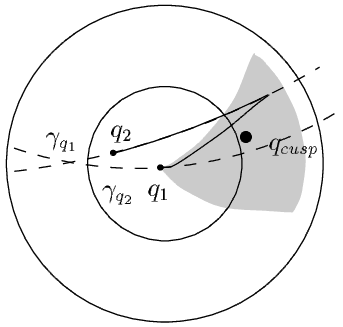
\includegraphics[width=0.5\textwidth]{img/steer.png}
	\end{figure}
\end{frame}

\begin{frame}{Chemin cinématique}
	\begin{itemize}
		\item Récursivement sur le chemin géométrique
		\item Si $\steerflat$ peut joindre les points (sans toucher
			d'obstactles), joindre
		\item Sinon, séparer en deux bouts et réappliquer
	\end{itemize}

	\vspace{1em}

	Phase de lissage~:

	\begin{itemize}
		\item Prendre aléatoirement des points d'arrêt
		\item Essayer de les joindre avec l'algorithme précédent
		\item Arrêt quand le nombre de points ne diminue plus
	\end{itemize}
\end{frame}

\begin{frame}{Trajectoire}
	\begin{itemize}
		\item Objectif~: trouver $s : \mathbb{R}_+ \to [0, 1]$ croissante
			(\og{}temps~\fg)
		\item $\forall t, q(t) = \gamma(s(t))$
		\item Représentation des contraintes sur les vitesses, accélérations
			dans le plan $(s, \dot{s})$
		\item Utilisation d'accélérations constantes par morceaux \og{}tant que
			possible~\fg{}
		\item Bon compromis optimalité-temps de calcul~: calcul embarqué sur
			Hilare
	\end{itemize}
\end{frame}

\end{document}
